% Figure of "Galashin's Conjecture 4.3 via a convex gradient": the local sign count behind eq:signed-excess in the
% strand-diagram proof of Proposition prop:wp. Typeset in the paper's own fonts (T1, Latin Modern, 11pt) at the
% paper's text width (6.5in), so \includegraphics does not rescale it. Schematic; it adds no assertion.
% Entries are filled points and exits open points; the first strand is blue and solid, the second ochre and dashed.
% Build: pdflatex <this file> && pdftocairo -svg <this file>.pdf <this file>.svg
\documentclass[11pt,border={0pt 4pt}]{standalone}
\usepackage[T1]{fontenc}
\usepackage{lmodern}
\usepackage{amsmath,amssymb}
\usepackage{tikz}
\usetikzlibrary{arrows.meta,calc}

% the palette of the paper's other figures
\definecolor{ink}{HTML}{233740}
\definecolor{muted}{HTML}{65757D}
\definecolor{pblue}{HTML}{0072B2}
\definecolor{qochre}{HTML}{B87827}

\begin{document}
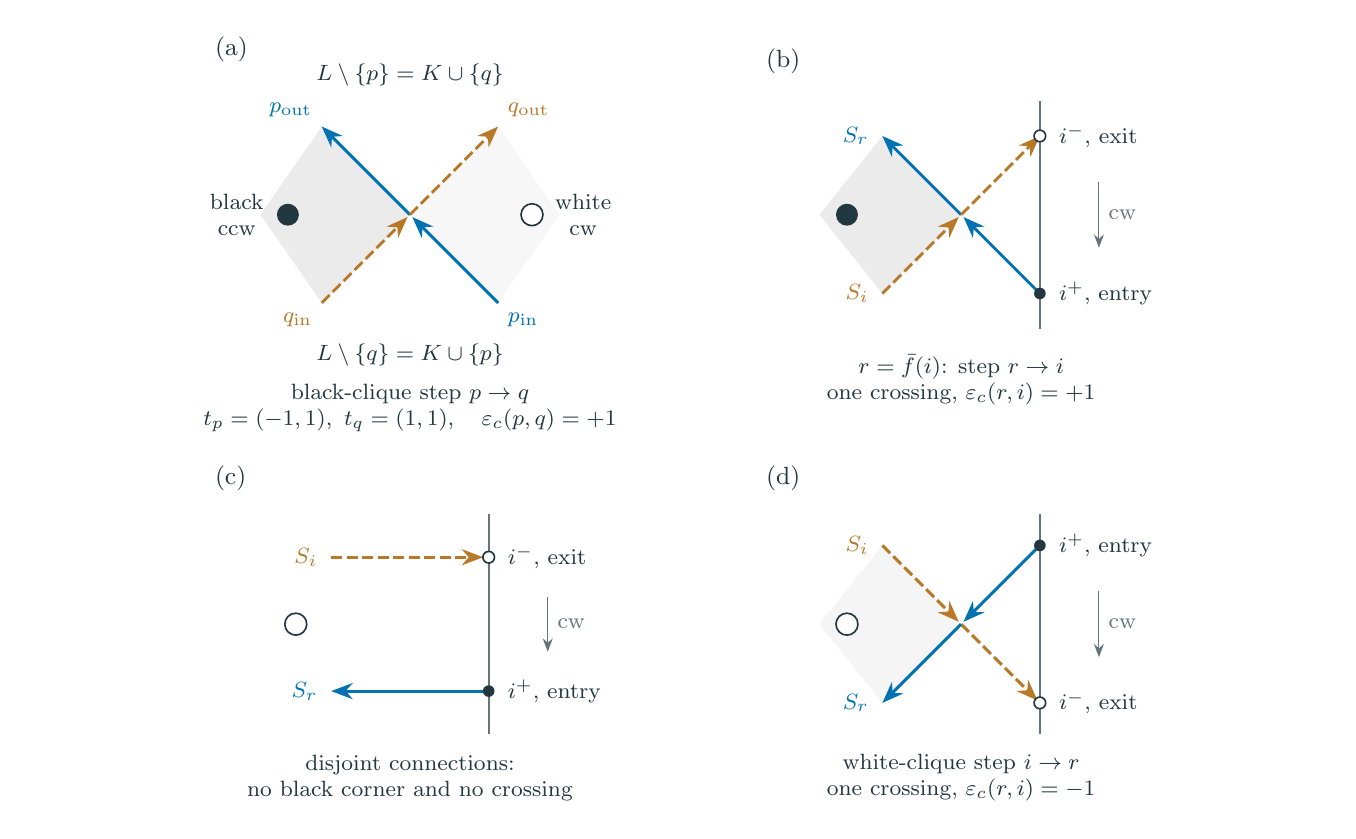
\begin{tikzpicture}[
  x=1cm,y=1cm,font=\small,>=Stealth,text=ink,
  p/.style={pblue,line width=1.05pt,->},
  q/.style={qochre,line width=1.05pt,->,dash pattern=on 4pt off 1.6pt},
  bd/.style={muted,line width=.6pt},
  blackv/.style={circle,fill=ink,inner sep=2.8pt},
  whitev/.style={circle,draw=ink,fill=white,line width=.6pt,inner sep=2.8pt},
  entry/.style={circle,fill=ink,inner sep=0pt,minimum size=4.2pt},
  exit/.style={circle,draw=ink,fill=white,line width=.6pt,inner sep=0pt,minimum size=4.2pt},
  lab/.style={font=\footnotesize},
  tag/.style={font=\small,anchor=west},
  note/.style={font=\footnotesize,align=center}
]
% (a) Interior chart: clockwise rays are p_out, q_out, p_in, q_in.
\begin{scope}
  \node[tag] at (-2.6,2.1) {(a)};
  \fill[black!8] (0,0)--(-1.12,1.12)--(-1.9,0)--(-1.12,-1.12)--cycle;
  \fill[black!3] (0,0)--(1.12,1.12)--(1.9,0)--(1.12,-1.12)--cycle;
  \node[blackv] at (-1.55,0) {};
  \node[whitev] at (1.55,0) {};
  \draw[p] (1.12,-1.12)--(.03,-.03);
  \draw[p] (0,0)--(-1.12,1.12);
  \draw[q] (-1.12,-1.12)--(-.03,-.03);
  \draw[q] (0,0)--(1.12,1.12);
  \node[lab,anchor=south east,text=pblue] at (-1.12,1.12) {$p_{\rm out}$};
  \node[lab,anchor=south west,text=qochre] at (1.12,1.12) {$q_{\rm out}$};
  \node[lab,anchor=north west,text=pblue] at (1.12,-1.12) {$p_{\rm in}$};
  \node[lab,anchor=north east,text=qochre] at (-1.12,-1.12) {$q_{\rm in}$};
  \node[lab] at (0,1.78) {$L\setminus\{p\}=K\cup\{q\}$};
  \node[lab] at (0,-1.78) {$L\setminus\{q\}=K\cup\{p\}$};
  \node[lab,align=center] at (-2.2,0) {black\\ccw};
  \node[lab,align=center] at (2.2,0) {white\\cw};
  \node[note] at (0,-2.45) {black-clique step $p\to q$\\
       $t_p=(-1,1),\ t_q=(1,1),\quad\varepsilon_c(p,q)=+1$};
\end{scope}
% (b) A black vertex next to the refined boundary.
\begin{scope}[xshift=7cm]
  \node[tag] at (-2.6,1.95) {(b)};
  \fill[black!8] (0,0)--(-1,1)--(-1.8,0)--(-1,-1)--cycle;
  \node[blackv] at (-1.45,0) {};
  \draw[bd] (1,-1.45)--(1,1.45);
  \draw[p] (1,-1)--(.03,-.03);
  \draw[p] (0,0)--(-1,1);
  \draw[q] (-1,-1)--(-.03,-.03);
  \draw[q] (0,0)--(1,1);
  \node[lab,anchor=east,text=pblue] at (-1.05,1) {$S_r$};
  \node[lab,anchor=east,text=qochre] at (-1.05,-1) {$S_i$};
  \node[exit] at (1,1) {};
  \node[entry] at (1,-1) {};
  \node[lab,anchor=west] at (1.12,1) {$i^-$, exit};
  \node[lab,anchor=west] at (1.12,-1) {$i^+$, entry};
  \draw[->,muted] (1.75,.42)--(1.75,-.42) node[midway,right,lab] {cw};
  \node[note] at (0,-2.1) {$r=\bar f(i)$: step $r\to i$\\
       one crossing, $\varepsilon_c(r,i)=+1$};
\end{scope}
% (c) A white neighbour: the same refined endpoints, no intersection.
\begin{scope}[yshift=-5.2cm]
  \node[tag] at (-2.6,1.85) {(c)};
  \node[whitev] at (-1.45,0) {};
  \draw[bd] (1,-1.4)--(1,1.4);
  \draw[q] (-1,.85)--(.93,.85);
  \draw[p] (1,-.85)--(-1,-.85);
  \node[lab,anchor=east,text=qochre] at (-1.05,.85) {$S_i$};
  \node[lab,anchor=east,text=pblue] at (-1.05,-.85) {$S_r$};
  \node[exit] at (1,.85) {};
  \node[entry] at (1,-.85) {};
  \node[lab,anchor=west] at (1.12,.85) {$i^-$, exit};
  \node[lab,anchor=west] at (1.12,-.85) {$i^+$, entry};
  \draw[->,muted] (1.75,.35)--(1.75,-.35) node[midway,right,lab] {cw};
  \node[note] at (0,-1.95) {disjoint connections:\\no black corner and no crossing};
\end{scope}
% (d) The other refinement, not used: entry before exit.
\begin{scope}[xshift=7cm,yshift=-5.2cm]
  \node[tag] at (-2.6,1.85) {(d)};
  \fill[black!4] (0,0)--(-1,1)--(-1.8,0)--(-1,-1)--cycle;
  \node[whitev] at (-1.45,0) {};
  \draw[bd] (1,-1.4)--(1,1.4);
  \draw[q] (-1,1)--(-.03,.03);
  \draw[q] (0,0)--(.97,-.97);
  \draw[p] (1,1)--(.03,.03);
  \draw[p] (0,0)--(-1,-1);
  \node[lab,anchor=east,text=qochre] at (-1.05,1) {$S_i$};
  \node[lab,anchor=east,text=pblue] at (-1.05,-1) {$S_r$};
  \node[entry] at (1,1) {};
  \node[exit] at (1,-1) {};
  \node[lab,anchor=west] at (1.12,1) {$i^+$, entry};
  \node[lab,anchor=west] at (1.12,-1) {$i^-$, exit};
  \draw[->,muted] (1.75,.42)--(1.75,-.42) node[midway,right,lab] {cw};
  \node[note] at (0,-1.95) {white-clique step $i\to r$\\
       one crossing, $\varepsilon_c(r,i)=-1$};
\end{scope}
% exactly the text width, 468 bp = 16.51 cm, centred on the drawing
\path let \p1=(current bounding box.center) in (\x1-8.255cm,\y1) -- (\x1+8.255cm,\y1);
\end{tikzpicture}
\end{document}
